\documentclass[math-font=newcm]{sjtuarticle}

\usepackage{enumitem}
\usepackage[hybrid,citations,fencedCode,underscores=false]{markdown}

\usepackage[style=gb7714-2015]{biblatex}
\addbibresource{ref.bib}

\graphicspath{{figs/}}

\usepackage{float}

\usepackage{listings}
\captionsetup[lstlisting]{labelfont=bf,justification=justified}
\providecommand{\code}[2]{\lstinputlisting[language=#2,caption=\href{run:#1}{\ttfamily #1}]{#1}}
\definecolor{grey}{rgb}{0.8,0.8,0.8}
\definecolor{darkgreen}{rgb}{0,0.3,0}
\definecolor{darkblue}{rgb}{0,0,0.3}
\lstset{%
    numbers=left, %行号
    numberstyle=\tiny\color{grey},
    showstringspaces=false,
    showspaces=false,%
    tabsize=4,%
    frame=shadowbox,%
    basicstyle={\ttfamily\small},%
    keywordstyle=\color{blue!80!black}\bfseries,%
    identifierstyle=,%
    commentstyle=\color{green!50!blue}\itshape,%
    stringstyle=\color{green!50!black},%
    rulesepcolor=\color{gray!20!white},
    breaklines,
    columns=flexible,
    extendedchars=false,
    mathescape=true,
    escapebegin=\color{green!50!blue}
}

\usepackage[linesnumbered,ruled]{algorithm2e}
\usepackage[colorlinks]{hyperref}

\title{作业1}
\author{Log Creative}
\date{2024 年 3 月 14 日}
\begin{document}
\maketitle

\tableofcontents*
\clearpage

\section{问题}

Design an incremental algorithm for the given polynomial:
\begin{equation}\label{eq:poly}
    y=ax^2+bx+c\quad(x_b\leq x\leq x_e)
\end{equation}
(without any multiplication)

\section{递增式算法}

\subsection{算法描述}

对于多项式 \eqref{eq:poly},可以得到横坐标相差1时纵坐标的差分值
\begin{equation}
    \increment y(x)=y(x+1)-y(x)=2ax+a+b
\end{equation}

当知道起始点$x_b$的纵坐标$y(x_b)$时,就可以通过差分值得到区间内任意一点的纵坐标
\begin{equation}\label{eq:tmpres}
    y(x)=y(x_b)+\sum_{i=0}^{x-x_b-1}\increment y(x_b+i)
\end{equation}

但是每次都计算差分值实际上会有一定的重复计算(当认为乘法计算代价高的时候),所以考虑使用二阶差分来进一步加速运算
\begin{equation}
    \increment[\increment y(x)]=2ax+a+b-[2a(x-1)+a+b]=2a=a+a
\end{equation}

那么式 \eqref{eq:tmpres} 就变成
\begin{equation}\label{eq:res}
    y(x)=y(x_b)+\sum_{i=0}^{x-x_b-1}[\increment y(x_b)+(a+a)i]
\end{equation}

或者写成迭代的形式
\begin{equation}
    y(x+1)=y(x)+\increment y(x)=y(x)+[\increment y(x-1)+(a+a)]
\end{equation}

就可以实现全加法的迭代运算。式 \eqref{eq:res} 提示我们需要预先知道 $y(x_b)$ 和 $\increment y(x_b)$,本文将会从 0 出发,使用累加的方式实现乘法,算出这两个初值,具体实现见第 \ref{sec:code} 节的 \verb"getValue(x)" 函数和 \verb"polyItem(coeff, base, order)" 函数。

\subsection{伪代码}

主要伪代码见算法 \ref{alg:incrpoly}。

\begin{algorithm}[H]
    \caption{递增式计算抛物线}
    \label{alg:incrpoly}
    \KwIn{多项式系数 $a,b,c$,起始点$x_b$,终止点$x_e$}
    \KwOut{区间 $[x_b,x_e]$ 对应的多项式结果 $\mathbf{y}$}
    \BlankLine
    使用累加计算 $y(x_b)=ax_b^2+bx_b+c$,$\increment y(x_b)=2ax_b+a_b$\;
    设定变量初值 $y\leftarrow y(x_b)$,$\increment y\leftarrow \increment y(x_b)$\;
    \ForEach{$x$\leftarrow $x_b$ to $x_e$}{
        $\mathbf{y}(x)\leftarrow \text{round}(y)$\;
        $y\leftarrow y+\increment y$\;
        $\increment y\leftarrow \increment y + a + a$\;
    }
    \Return{$\mathbf{y}$}\;
\end{algorithm}

\subsection{代码实现}\label{sec:code}

代码实现于 \verb"IncrPoly" 类中,算法 \ref{alg:incrpoly} 主要实现于 \verb"getRangeValue()" 函数,它会调用 \verb"getValue(x)" 来计算初值,这两个函数都会调用 \verb"polyItem(coeff, base, order)" 函数来计算单个多项式项的值。

其中 \verb"polyItem"$(a,x,r)$ 采用累加、迭代的形式实现对多项式项 $ax^r$ 的计算:对于高阶项($r>1$)会逐步化归为1阶的情况,对于1阶的情况,采用从0的位置开始逐步累加(减)浮点数的形式得到对应的值。
\begin{equation}
    ax^r=\texttt{polyItem}(a,x,r)=\begin{cases}
        a, & r=0;\\
        \underbrace{a+\cdots+a}_{\#a=x} , & r=1\text{ and }x\geq 0;\\
        \underbrace{-a-\cdots-a}_{\#a=x} ,  & r=1\text{ and }x<0;\\
        \texttt{polyItem}(ax^{r-1},x,1), & r>1.
    \end{cases}
\end{equation}

\code{../source/IncrPoly/IncrPoly.hpp}{c++}

\section{命令行程序}

\subsection{运行方式}\label{sec:cliinput}

\begin{figure}[h]
    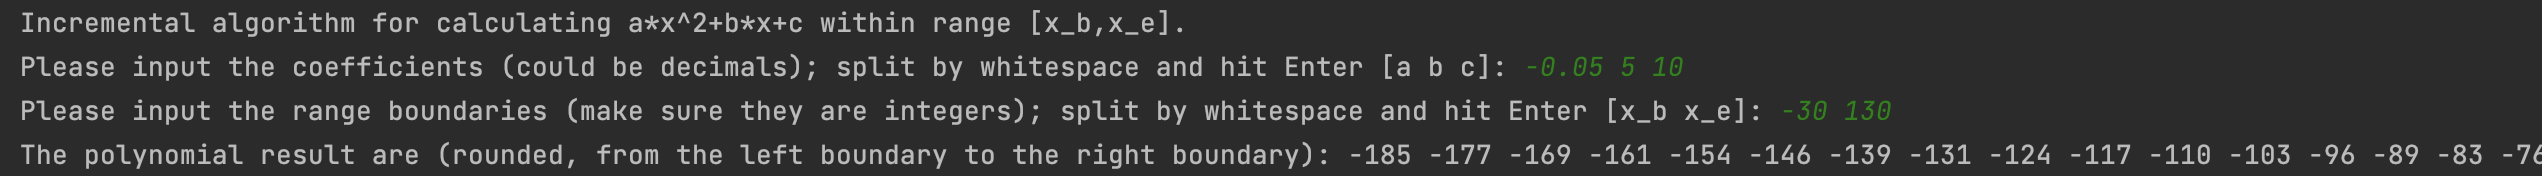
\includegraphics[width=\textwidth]{cli.png}
    \caption{命令行程序输出结果}\label{fig:cli}
\end{figure}

运行命令行程序,如图 \ref{fig:cli} 所示。首先输入三个参数(用空格分隔),比如 \verb"-0.05 5 10",按下回车;接着输入左右边界(用空格分隔,如果输入不是整数,将会转换为整数),比如 \verb"-30 130",按下回车;最后就会输出这个区间之间纵坐标的整数结果。

\subsection{代码实现}

命令行程序的代码展示了如何基本地调用 \verb"IncrPoly" 类。

\code{../source/IncrPoly/main.cpp}{c++}

\lstset{basicstyle=\ttfamily\scriptsize}

其中 \verb"IncrPoly-cli.h" 主要实现了终端输入提示逻辑。

\code{../source/IncrPoly/IncrPoly-cli.h}{c++}

\section{OpenGL展示}

\subsection{运行方式}

\begin{figure}[h]
    \centering
    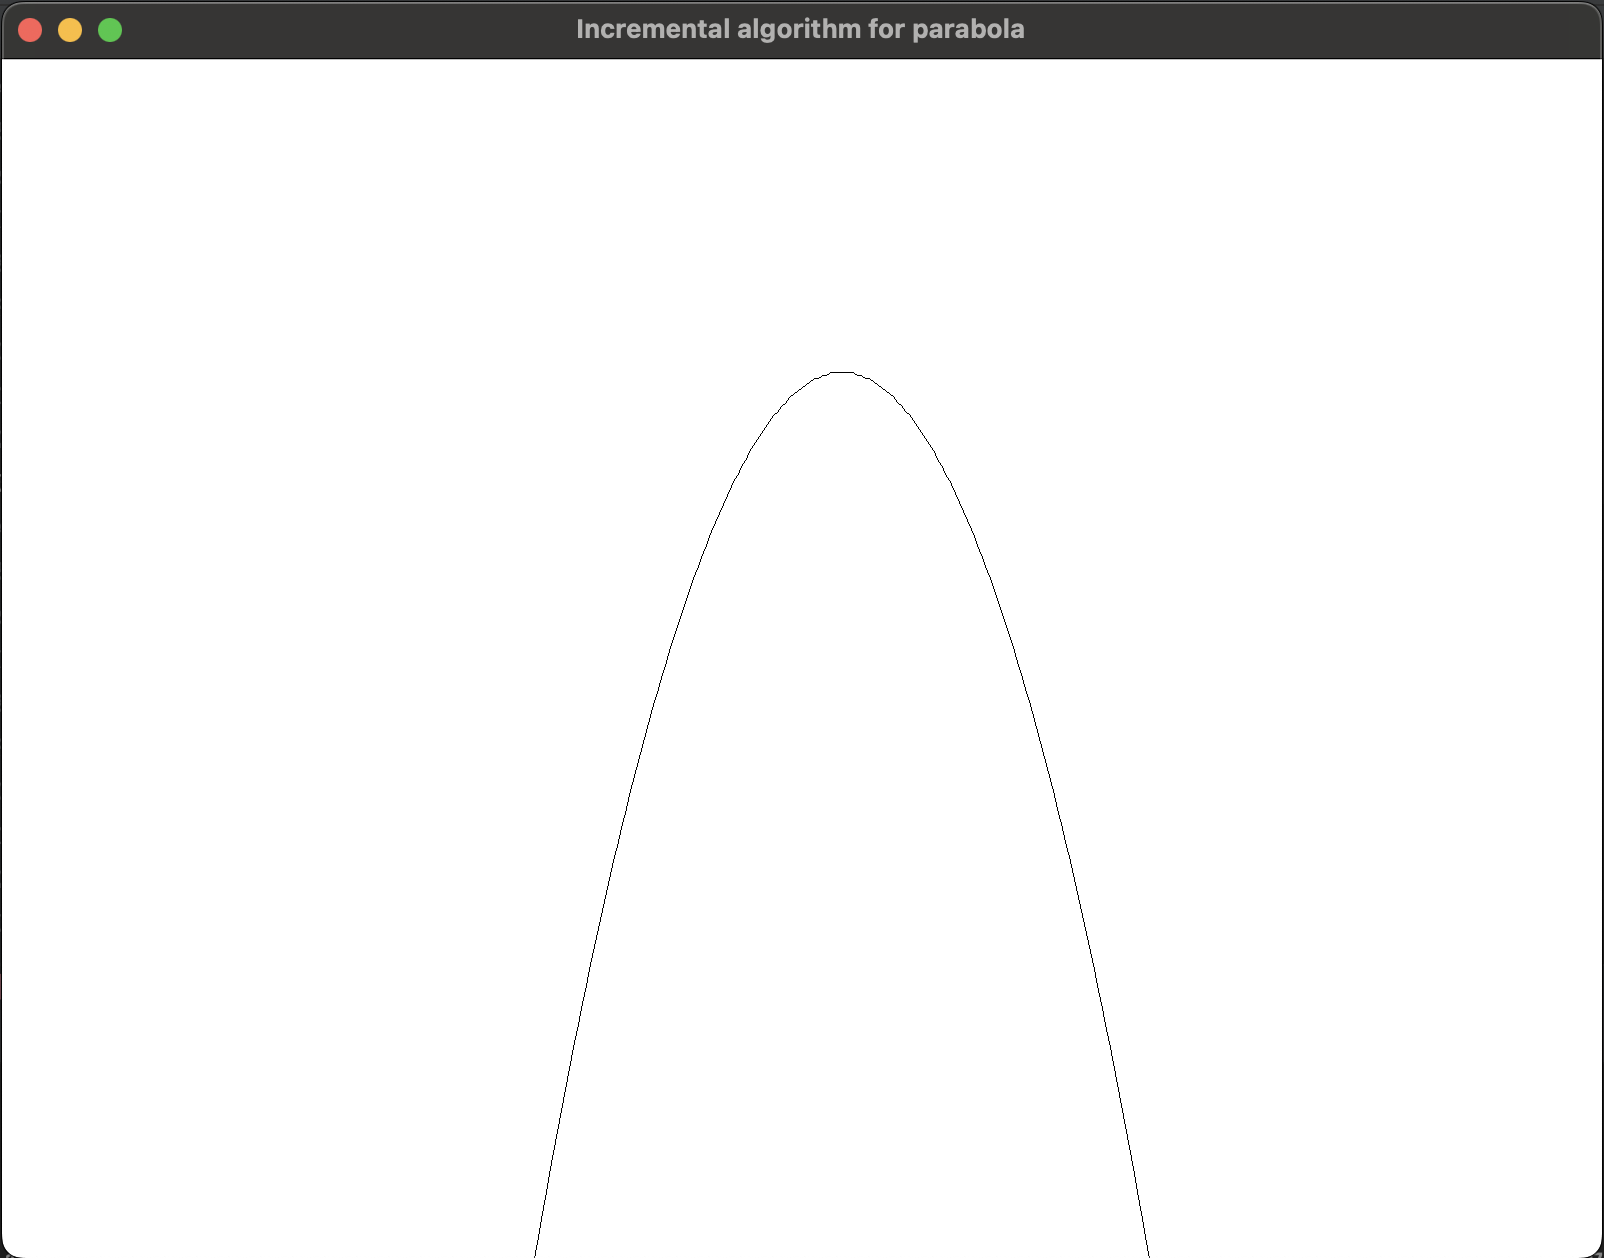
\includegraphics[width=0.7\textwidth]{gui.png}
    \caption{图形程序输出结果,输入 $a=-0.05,b=5,c=10,x_b=-30,x_e=130$}\label{fig:gui}
\end{figure}

运行图形程序,按照第 \ref{sec:cliinput} 节的终端输入方法输入相关数值,然后就可以在弹出的窗口中看到如图 \ref{fig:gui} 所示的可视化结果。


\subsection{代码实现}

基本框架对照 LearnOpenGL《你好,三角形》一节\cite{hellotri} 设置,其中头文件 \verb"shader_s.h" 中的着色器类为 LearnOpenGL 《着色器》一节\cite{shaders} 的源代码\cite{shadersrc},会加载顶点着色器 \verb"vertexShader.glsl" 和片段着色器 \verb"fragmentShader.glsl"。

\code{../source/src/main.cpp}{c++}

\code{../source/assets/shader/vertexShader.glsl}{c}

\code{../source/assets/shader/fragmentShader.glsl}{c}

\printbibliography[heading=bibintoc]

\appendix

\lstset{basicstyle={\ttfamily\small}}

\markdownInput{../executable/README.md}

\markdownInput{../source/README.md}

\end{document}